%%
%% GSHAC — arXiv preprint
%% Compile: pdflatex -> bibtex -> pdflatex -> pdflatex
%%
%% ---------------------------------------------------------------------------
%% STAGE SWITCHER (change this one line to move between stages):
%%   arXiv preprint (current):  [manuscript, screen, review]
%%   ACM submission:            [sigconf, review]
%%   Camera-ready / TAPS:       [sigconf]
%% ---------------------------------------------------------------------------
\documentclass[sigconf, screen]{acmart}

% ---------------------------------------------------------------------------
% Suppress ACM auto-generated blocks (useful for arXiv/preprint versions).
% NOTE: For an ACM camera-ready submission you should NOT disable these.
% ---------------------------------------------------------------------------
\settopmatter{printacmref=false} % removes "ACM Reference Format" block
\renewcommand\footnotetextcopyrightpermission[1]{} % removes permission footnote text
\setcopyright{none} % removes copyright/permission strip entirely

%% ---------------------------------------------------------------------------
%% ACM rights block — leave commented for arXiv.
%% Fill in the values provided in the ACM rights-confirmation e-mail and
%% uncomment for camera-ready / TAPS submission.
%% ---------------------------------------------------------------------------
%% \setcopyright{acmlicensed}
%% \acmDOI{XXXXXXX.XXXXXXX}
%% \acmISBN{978-1-4503-XXXX-X/2026/11}
%%
%% Conference metadata (keep for all stages; update acronym/dates if needed)
% \acmConference[SIGSPATIAL '26]{34th ACM SIGSPATIAL International Conference on Advances in Geographic Information Systems}{November 2026}{Atlanta, Georgia, USA}
% \acmYear{2026}
% \copyrightyear{2026}


%% Packages
\usepackage{algorithm}
\usepackage{algpseudocode}
\usepackage{booktabs}
\usepackage{multirow}
\usepackage{graphicx}
\usepackage{microtype}
\usepackage{enumitem}
\let\Bbbk\relax          % newtxmath (loaded by acmart) already defines \Bbbk
\usepackage{amsmath,amssymb,amsthm}
\usepackage{xcolor}
\usepackage{url}

%% Theorem environments
\newtheorem{theorem}{Theorem}
\newtheorem{proposition}[theorem]{Proposition}
\newtheorem{corollary}[theorem]{Corollary}
\newtheorem{definition}{Definition}

%% Convenience
\newcommand{\hmax}{h_{\max}}
\newcommand{\Onotation}[1]{\mathcal{O}\!\left(#1\right)}

% -----------------------------------------------------------------------
\begin{document}

\title{Scalable Exact Hierarchical Agglomerative Clustering via \\ Sparse Geographic Distance Graphs}

\author{Victor Maus}
\orcid{https://orcid.org/0000-0002-7385-4723}
\affiliation{%
  \institution{WU Vienna University of Economics and Business}
  \city{Vienna}
  \country{Austria}
}
\email{victor.maus@wu.ac.at}

\author{Vinicius Pozzobon Borin}
%\orcid{https://orcid.org/XXXX-XXXX-XXXX-XXXX}
\affiliation{%
  \institution{University of Oulu}
  \city{Oulu}
  \country{Finland}
}
\email{vinicius.borin@oulu.fi}

% -----------------------------------------------------------------------
\begin{abstract}
Exact hierarchical agglomerative clustering (HAC) of large spatial datasets is limited in practice by the \(\Onotation{n^2}\) time and memory required for the full pairwise distance matrix. We present \emph{GSHAC} (Geographically Sparse Hierarchical Agglomerative Clustering), a system that makes exact HAC for geographic data feasible at scales of millions of features on a commodity workstation. We replace the distance matrix with a sparse geographic distance graph containing only pairs within a user-specified geodesic bound~\(\hmax\). The graph is constructed in \(\Onotation{n \cdot k}\) time via spatial indexing (KD-tree or Ball-tree), where~\(k\) is the mean number of neighbors within~\(\hmax\), and its connected components define independent subproblems for standard HAC. We prove that the resulting cluster assignments are \emph{exact} when compared to those from a dense matrix for all standard linkage methods at any cut height \(h \le \hmax\). For single linkage, an MST-based path avoids dense sub-matrices entirely, keeping memory in \(\Onotation{n_k + m_k}\) per component regardless of component size. Applied to a global mining inventory (\(n = 261{,}073\) features)~\cite{maus2026data}, the system completes in 12\,s on a commodity laptop (109\,MiB peak HAC memory; \(121\,\text{MB}\) graph storage) whereas the dense baseline would require \(\approx\!545\,\text{GB}\), unfeasible on the laptop. On a 2-million-point sample of GeoNames (global named places), four tested thresholds completed in under 3\,minutes each with peak memory under 3\,\text{GB}. To our knowledge, these are the largest demonstrations of exact HAC on geographic data on a single workstation, opening the door for applied researchers and practitioners to analyze geographic data with millions of features using substantially reduced resources. We provide an implementation compatible with Python's scikit-learn that enables direct integration into GIS workflows.
\end{abstract}

% CCS concepts
\begin{CCSXML}
<ccs2012>

   <concept>
       <concept_id>10002951.10003227.10003351.10003444</concept_id>
       <concept_desc>Information systems~Clustering</concept_desc>
       <concept_significance>500</concept_significance>
    </concept>
       
   <concept>
       <concept_id>10002951.10003227.10003236.10003237</concept_id>
       <concept_desc>Information systems~Geographic information systems</concept_desc>
       <concept_significance>500</concept_significance>
    </concept>
       
   <concept>
       <concept_id>10003752.10003809</concept_id>
       <concept_desc>Theory of computation~Design and analysis of algorithms</concept_desc>
       <concept_significance>300</concept_significance>
       </concept>
   
   <concept>
       <concept_id>10010147.10010257</concept_id>
       <concept_desc>Computing methodologies~Machine learning</concept_desc>
       <concept_significance>300</concept_significance>
    </concept>
    
 </ccs2012>
\end{CCSXML}

\ccsdesc[500]{Information systems~Clustering}
\ccsdesc[500]{Information systems~Geographic information systems}
\ccsdesc[300]{Theory of computation~Design and analysis of algorithms}
\ccsdesc[300]{Computing methodologies~Machine learning}


\keywords{hierarchical clustering, spatial data, sparse distance graph, geographic locality, spatial index, scalable algorithm, fastclusters, scikit-learn}

\maketitle

%% ---------------------------------------------------------------------------
%% Preprint notice — remove this block for ACM submission / camera-ready
%% ---------------------------------------------------------------------------
% \begin{quote}
% \small\itshape
% Preprint. Submitted to the 34th ACM SIGSPATIAL International Conference on Advances in Geographic Information Systems (ACM SIGSPATIAL 2026). This version is deposited on arXiv in accordance with ACM's author rights policy.
% \end{quote}

% =======================================================================

%\tableofcontents

\section{Introduction}
\label{sec:intro}

%Widely used in spatial analysis \cite{sadeghi2025clustering}, Hierarchical Agglomerative Clustering (HAC) is a fundamental unsupervised machine learning technique for uncovering the inherent nested structure of datasets. Unlike partitional methods such as K-Means, which require the number of clusters to be specified in advance and assume spherical cluster shapes, HAC provides a rich, multi-resolution dendrogram that can be cut at arbitrary levels \cite{sadeghi2025clustering}.

%Despite its analytical power, the practical application of exact HAC to large datasets is bottlenecked by its computational requirements. Standard HAC algorithms necessitate the computation and storage of a full pairwise distance matrix, resulting in an $\mathcal{O}(n^2)$ memory and time complexity \cite{nguyen2014sparsehc, mullner2013fastcluster}. For large geographic databases containing millions of features, this quadratic scaling is prohibitive, routinely exceeding the RAM limits of standard workstations and forcing practitioners to rely on data downsampling, approximate heuristics, or less informative partitional algorithms \cite{sadeghi2025clustering, gagolewski2016genie}. XXXXXXXXX.

Hierarchical Agglomerative Clustering (HAC) is a fundamental unsupervised learning technique widely used across numerous scientific disciplines because it provides an informative, multi-scale representation of data structure without requiring a predefined number of clusters \cite{mullner2013fastcluster}. In spatial analysis and geo-data science, HAC is highly valued for exploratory data analysis, geochemical anomaly detection, and discovering nested regional structures \cite{sadeghi2025clustering}. Unlike partitional methods such as K-Means, which require the number of clusters to be specified in advance and assume spherical cluster shapes, HAC provides a rich, multi-resolution dendrogram that can be cut at arbitrary levels \cite{sadeghi2025kmeans}.

Despite its analytical utility, standard HAC suffers from severe scalability bottlenecks. Constructing the hierarchical dendrogram traditionally requires calculating and storing a full pairwise distance matrix, which imposes an \(\mathcal{O}(n^2)\) memory footprint and an \(\mathcal{O}(n^3)\) or \(\mathcal{O}(n^2log~n)\) time complexity \cite{nguyen2014sparsehc, gagolewski2016genie}. This quadratic wall renders exact HAC computationally infeasible for large modern datasets on commodity hardware \cite{hendrix2013scalable}.

To overcome these limitations and allow scalable applications, a variety of approaches have been proposed across different fields. Methods such as BIRCH and CURE utilize data summarization (e.g., CF-trees) or random sampling with multiple representatives to approximate the hierarchy in a single or a few passes \cite{zhang1996birch, guha1998cure}. For single-linkage clustering, distributed and parallel computing architectures, such as MapReduce and Message Passing Interface (MPI), have been leveraged to partition the Minimum Spanning Tree (MST) computation across multiple nodes \cite{jin2015incremental, hendrix2013scalable}. In general metric spaces, algorithms have incorporated Approximate Nearest Neighbor (ANN) data structures and Locality Sensitive Hashing (LSH) to achieve subquadratic runtimes by trading exactness for speed \cite{moseley2020hierarchical}. Additionally, memory-efficient online algorithms like SparseHC process distance matrices in a chunk-by-chunk manner, exploiting sparsity to reduce memory consumption for biological data \cite{nguyen2014sparsehc} but require a pre-computed sparse matrix.

For geographic data specifically, variants of HAC have been effectively applied, such as the spatial-constraints Ward-like algorithm proposed in \cite{chavent2018clustgeo}. Furthermore, Maus (2026) recently proposed a graph-indexing method to compute sparse pairwise distances for HAC suitable for large spatial datasets \cite{maus2026data}. By applying a maximum spatial distance threshold, the method partitions geographic features into independent groups that can be computed efficiently with low memory requirements \cite{maus2026data}. However, this work has a strict application focus on mining land use and does not provide formal mathematical proofs that the approach generalizes across different standard linkage methods, nor does it prove that it strictly reduces computing time and memory bounds.

In this paper, we present GSHAC (Geographically Sparse Hierarchical Agglomerative Clustering), a system that makes exact HAC for multiple linkage methods feasible for millions of geographic features on commodity hardware. The system leverages the First Law of Geography (``Everything is related to everything else, but near things are more related than distant things''~\cite{tobler1970computer}), which implies that, in spatial and geographic contexts, features separated by vast geographic distances are highly unlikely to merge until the very final stages of 
the hierarchical tree. Therefore, rather than computing a dense distance matrix, GSHAC leverages spatial indexing (e.g., KD-trees~\cite{bentley1975quad} and Ball Trees~\cite{omohundro1989balltree}) to construct a sparse 
geographic distance graph in $\mathcal{O}(n(\log n + k))$ time, where $k$ is the mean number of neighbors within a user-specified geodesic threshold $h_{\max}$. In practice, when the sparsity assumption holds, that is, when $k \gg \log n$, this reduces to $\mathcal{O}(n \cdot k)$, which remains linear in $n$ for fixed $k$. We formally prove that the connected components of this sparse graph constitute independent subproblems, guaranteeing that the resulting cluster assignments are strictly exact for all standard linkage methods at any cut height $h \leq h_{\max}$. We make the following contributions:

\begin{enumerate}

  \item A system design that combines spatial indexing, connected-component decomposition, and MST-based single-linkage into a practical pipeline for exact HAC on geographical data at scales. We provide a proof that this approach is exact for all standard linkage methods (single, complete, average, Ward) at any cut height \(h \le \hmax\).
  
  \item Empirical evaluation at four datasets: a synthetic dataset with (\(n\) up to \(100{,}000\)), the Iris dataset, and two real-world sets, a mining dataset (\(n = 261{,}073\)) \cite{maus2026data} and location names from GeoNames (\(n = 2{,}000{,}000\)) \cite{geonames2025}.

  \item An open-source Python implementation with a scikit-learn-compatible \texttt{SpatialAgglomerativeClustering} estimator \url{https://github.com/mine-the-gap/gshac}.

\end{enumerate}

\section{Related work}

\textbf{Exact HAC and Classical Bottlenecks} 

Standard implementations of HAC, such as the widely used \texttt{fastcluster} package for R and Python \cite{mullner2013fastcluster}, provide highly optimized routines for standard linkage criteria (e.g., single, complete, average, Ward). However, these exact algorithms are still fundamentally limited by $\mathcal{O}(n^2)$ memory requirements when processing dense dissimilarity matrices \cite{mullner2013fastcluster}. In geo-data science, frameworks such as ClustGeo \cite{chavent2018clustgeo} incorporate spatial constraints by combining a feature distance matrix with a geographic distance matrix using a mixing parameter. While effective for identifying spatially contiguous clusters, these methods retain the $\mathcal{O}(n^2)$ cost of dense matrix operations, limiting their applicability to smaller regional datasets \cite{chavent2018clustgeo}.

\textbf{Single Linkage and Minimum Spanning Trees}

The mathematical equivalence between single-linkage clustering and the Minimum Spanning Tree (MST) has long been established \cite{gower1969minimum}. Algorithms such as SLINK compute the single-linkage hierarchy in optimal $\mathcal{O}(n^2)$ time and $\mathcal{O}(n)$ space \cite{sibson1973slink}. Recent advances have introduced fast parallel algorithms for Euclidean MSTs (EMST) using Well-Separated Pair Decompositions and KD-trees \cite{wang2021fast}. While these parallel methods can cluster tens of millions of points efficiently, they generally require distributed systems or massive multi-core hardware instances with hundreds of gigabytes of RAM \cite{wang2021fast}. 

\textbf{Sparse and Cutoff-Based Clustering}

To mitigate memory issues, algorithms like SparseHC \cite{nguyen2014sparsehc} process distance matrices chunk-by-chunk using a predefined distance cutoff, ensuring exact dendrograms up to that threshold \cite{nguyen2014sparsehc}. However, SparseHC requires the input data to be pre-sorted and is restricted to specific linkage types (single, complete, average) \cite{nguyen2014sparsehc}. 

\textbf{Scalable and Approximate Hierarchical Clustering}

When exactness is relaxed, several highly scalable hierarchical algorithms exist. The Sub-Cluster Component (SCC) algorithm \cite{monath2021scalable} and the Tree Grafting (Grinch) method \cite{monath2019scalable} build hierarchies over billions of points. Grinch uses local rotations and global graft operations to dynamically restructure the tree, whereas SCC uses independent sub-cluster merging \cite{monath2021scalable}. However, these algorithms generally produce non-binary trees or heuristic structures that do not perfectly approximate exact HAC unless highly restrictive mathematical conditions are met \cite{monath2021scalable}. Similarly, the Genie algorithm \cite{gagolewski2016genie} adjusts the standard linkage criteria using a Gini-index to prevent the chaining effect and resist outliers, but it alters the classical HAC definitions and can still incur long computation times on standard machines compared to simple geometric bounds \cite{gagolewski2016genie}.

\textbf{Density-Based Spatial Clustering}

In geographic domains, algorithms like HDBSCAN \cite{mcinnes2017hdbscan} and OPTICS \cite{ankerst1999optics} natively exploit spatial sparsity and density to group points efficiently. While these density-based methods are highly effective for spatial anomaly detection and noise handling, they solve a fundamentally different objective than classical HAC \cite{ankerst1999optics}.

\textbf{Spatial Clustering Tools}

A recent review~\cite{sadeghi2025clustering} identifies hierarchical approaches as important for scale-sensitive spatial analysis, yet current tools remain limited by the \(\Onotation{n^2}\) bottleneck. scikit-learn's \texttt{Agglomerative\-Clustering}, for instance, supports a sparse \texttt{connectivity} parameter \cite{pedregosa2011sklearn} that constrains which pairs may merge, but it still computes pairwise distances internally and does not provide the component-wise decomposition needed for scalable distance-threshold HAC at large~\(n\).

\texttt{libpysal.weights.DistanceBand} from PySAL \cite{rey2007pysal} constructs sparse spatial weight matrices from distance thresholds using KD-trees, but stores binary or inverse-distance weights rather than actual geographic distances, and provides no exact HAC implementation. ClustGeo \cite{chavent2018clustgeo} extends Ward clustering with spatial constraints but requires the full \(\Onotation{n^2}\) distance matrix and has been demonstrated only for \(n \lesssim 10^3\).

A complementary line of recent work in ACM TSAS targets scalability for spatial clustering through different mechanisms than ours. PAGE~\cite{alrashid2023page} parallelises spatially-constrained regionalization for large polygon datasets via heuristic search subject to user-defined region constraints; its output is a single non-hierarchical partition optimised under a maximum-region constraint, whereas GSHAC produces an exact dendrogram cuttable at any height \(h \le \hmax\). HierGP~\cite{oje2025hiergp} achieves scale through hierarchical grid partitioning with user-controlled accuracy bounds, trading data fidelity for analytical throughput; GSHAC takes the opposite trade-off, processing every original feature without aggregation while exploiting geographic sparsity in the distance graph. Bicriteria Shapes~\cite{rottmann2025bicriteria} produces a hierarchically nested sequence of polygon aggregations parameterised by a perimeter--area bicriteria optimisation solved via graph cuts; like GSHAC it serves multi-scale-of-detail analyses, but optimises a different objective (shape compactness vs.\ distance threshold) and operates on polygon geometries rather than on a generic distance graph.

%GSHAC bridges the gap between these two domains, bringing the spatial indexing advantages typically reserved for density-based algorithms into the exact HAC ecosystem.


% \section{Related Work}
% \label{sec:related-work}

% This work focuses on how to perform HAC on large datasets (n\~millions) using a standard commodity workstation, and, to the maximum extent possible, avoid moving to distributed implementations, which can scale further but introduce infrastructure costs. Therefore, we do not provide a comprehensive overview of all available approaches and parallelization; we rather highlight what is available to users, especially for GIS analysis. The related work presented in this section provides an overview of the strengths and limitations of clustering algorithms and implementations readily available and commonly used by GIS users.

% \subsection{Clustering Scalability on a Workstation}

% HAC uses a dendrogram to iteratively merge the two closest clusters according to a linkage criterion. Standard methods include single (minimum inter-cluster distance), complete (maximum), average (UPGMA), and Ward (minimum variance). The naive implementation runs in \(\Onotation{n^2}\) time and requires the full \(n \times n\) distance matrix. \texttt{SLINK} \cite{sibson1973} solves single linkage in \(\Onotation{n^2}\) time with \(\Onotation{n}\) memory, but does not generalize to other linkages. Müllner's \texttt{fastcluster} \cite{mullner2013} achieves \(\Onotation{n^2}\) for all linking methods but still requires the full matrix.

% Approximate HAC \cite{monath2019} builds dendrograms over approximate neighbor graphs and does not preserve correctness at all cut heights {\color{red}WHAT IS THE TIME AND MEMORY COMPLEXITY OF APPROXIMATIONS? This paragraph needs expansion...} 

% The bioinformatics community has developed exact HAC algorithms that operate on pre-built sparse distance matrices. SparseHC \cite{nguyen2014sparsehc} scans a pre-sorted sparse matrix online, supporting single, complete, and average linkage with memory proportional to the stored distances. MC-UPGMA \cite{loewenstein2008mcupgma} proves exact UPGMA from a sparse similarity graph and demonstrates clustering of the UniRef90 protein database (\(n \approx 1.8\,\text{M}\)) on a single workstation. Both methods assume the sparse matrix is provided as input; neither addresses how to construct it efficiently, especially for spatial coordinates, which fall outside the scope of bioinformatics.

% A well-known result due to Gower and Ross \cite{gower1969} and Sibson \cite{sibson1973} establishes that the single-linkage dendrogram is equivalent to the minimum spanning tree (MST) of the complete distance graph. MST enables, for instance, HDBSCAN \cite{mcinnes2017hdbscan} to produce a fast density-based cluster tree that avoids the full \(\Onotation{n^2}\) matrix via Dual-Tree Bor\r{u}vka. Wang et al. \cite{wang2021emst} present parallel exact Euclidean MST and HDBSCAN at tens of millions of points, but require multi-core machines. An alternative linkage method, Genie \cite{gagolewski2016genie,gagolewski2021genieclust}, achieves near-linear empirical complexity for Euclidean data without pre-computing the full distance matrix. Neither Genie nor HDBSCAN provides an exact equivalent to standard HAC: HDBSCAN clusters reflect density rather than distance thresholds, while Genie is a modified single linkage approach that does not replace all HAC linkage methods.

% \subsection{Spatial Clustering Tools}
% % \label{sec:related_spatial}

% A recent review~\cite{sadeghi2025clusteringgeodata} identifies hierarchical approaches as important for scale-sensitive spatial analysis, yet current tools remain limited by the \(\Onotation{n^2}\) bottleneck. scikit-learn's \texttt{Agglomerative\-Clustering}, for instance, supports a sparse \texttt{connectivity} parameter \cite{pedregosa2011sklearn} that constrains which pairs may merge, but it still computes pairwise distances internally and does not provide the component-wise decomposition needed for scalable distance-threshold HAC at large~\(n\).

% PySAL's \texttt{libpysal.weights.DistanceBand} \cite{rey2007pysal} constructs sparse spatial weight matrices from distance thresholds using KD-trees, but stores binary or inverse-distance weights rather than actual geographic distances, and provides no exact HAC implementation. ClustGeo \cite{chavent2018clustgeo} extends Ward clustering with spatial constraints but requires the full \(\Onotation{n^2}\) distance matrix and has been demonstrated only for \(n \lesssim 10^3\).

\section{Theoretical formulation}
\label{sec:theoretical}

\subsection{Problem}
\label{sec:problem}

Let \(\mathcal{X} = \{x_1, \ldots, x_n\}\) be a set of~\(n\) spatial features with pairwise distance function~\(d: \mathcal{X} \times \mathcal{X} \to \mathbb{R}_{\ge 0}\) (geodesic or projected Euclidean). Let \(\hmax \in \mathbb{R}_{>0}\) be a user-specified maximum clustering distance, and \(H = \{h_1, \ldots, h_T\}\) with \(h_t \le \hmax\) be the
cut heights at which cluster assignments are required.

\begin{definition}[Geographic distance graph]
The geographic distance graph at radius~\(\hmax\) is the weighted undirected graph \(G_{\hmax} = (\mathcal{X}, E, w)\) where \(E = \{(i,j) : d(x_i, x_j) \le \hmax\}\) and \(w(i,j) = d(x_i, x_j)\).
\end{definition}

\begin{definition}[Connected component]
A connected component of~\(G_{\hmax}\) is a maximal set of features \(\mathcal{C} \subseteq \mathcal{X}\) such that every pair in~\(\mathcal{C}\) is connected by a path of edges in~\(E\).
\end{definition}

The goal is to compute, for each \(h \in H\), the same cluster assignment that would result from running HAC on the full dense distance matrix~\(D\), while computing and storing only the entries of~\(D\) corresponding to edges in \(G_{\hmax}\).

\subsection{Algorithm}
\label{sec:algorithm}

Algorithm~\ref{alg:main} has four phases: (i)~spatial index construction, (ii)~candidate pair discovery via range queries and exact distance computation, (iii)~connected component decomposition, and (iv)~independent HAC within each component. The key departure from the dense baseline is that only \(|E| = \Onotation{n \cdot k}\) distances are computed and stored, where \(k = |E| / n\) is the mean node degree in~\(G_{\hmax}\).

\begin{algorithm}[!h]
\caption{SparseGeoHClust}
\label{alg:main}
\begin{algorithmic}[1]
  \Require Features $\mathcal{X} = \{x_1,\ldots,x_n\}$, max distance
    $\hmax$, linkage method $\ell$, cut heights $H$
  \Ensure Cluster label vectors $\{\mathbf{c}^{(h)}\}_{h \in H}$

  \State Build spatial index $\mathcal{T}$ over $\mathcal{X}$
    \Comment{\(\Onotation{n \log n}\)}
  \State $E \leftarrow \emptyset$,\quad $\mathbf{S} \leftarrow$ empty sparse matrix
  \For{$i = 1$ \textbf{to} $n$}
    \State $N_i \leftarrow \mathcal{T}.\textsc{RangeQuery}(x_i, \hmax)$
      \Comment{spatial index lookup}
    \For{$j \in N_i$ with $j > i$}
      \Comment{upper triangle only}
      \State $s_{ij} \leftarrow d(x_i, x_j)$
        \Comment{exact distance}
      \State $\mathbf{S}[i,j] \leftarrow s_{ij}$;\quad
             $\mathbf{S}[j,i] \leftarrow s_{ij}$
             \Comment{symmetric}
      \State $E \leftarrow E \cup \{(i,j)\}$
    \EndFor
  \EndFor
  \State $\{\mathcal{C}_1,\ldots,\mathcal{C}_K\} \leftarrow
    \textsc{ConnectedComponents}(\mathbf{S})$
  \State Initialise label arrays $\mathbf{c}^{(h)}$ for all $h \in H$
  \State $g \leftarrow 0$ \Comment{global cluster ID counter}
  \For{$k = 1$ \textbf{to} $K$}
    \State $\mathbf{D}_k \leftarrow$ dense sub-matrix of $\mathbf{S}$ for $\mathcal{C}_k$
    \State $\Delta_k \leftarrow \textsc{hclust}(\mathbf{D}_k,\, \ell)$
      \Comment{standard HAC}
    \For{$h \in H$}
      \State $\mathbf{c}^{(h)}[\mathcal{C}_k] \leftarrow
        g + \textsc{CutTree}(\Delta_k, h)$
    \EndFor
    \State $g \leftarrow g + |\mathcal{C}_k|$
  \EndFor
  \State \textbf{return} $\{\mathbf{c}^{(h)}\}_{h \in H}$
\end{algorithmic}
\end{algorithm}



\subsection{Correctness}
\label{sec:correctness}

\paragraph{Intuition.}
The proof rests on a single observation: no merge at height \(h \le \hmax\) can involve features from different connected components, because all cross-component pairs have distance \(> \hmax\) by definition. The argument for each linkage method follows directly:
\begin{itemize}[leftmargin=*,topsep=2pt,itemsep=1pt]

  \item \emph{Single linkage}: the merge height equals the minimum inter-cluster distance; all cross-component minima exceed \(\hmax\).
  
  \item \emph{Complete linkage}: the merge height equals the maximum inter-cluster distance, at least as large as the minimum.
  
  \item \emph{Average linkage}: the merge height is the mean over all cross-cluster pairs, which exceeds \(\hmax\) when every pair does.
  
  \item \emph{Ward linkage}: the variance increase is monotone in inter-cluster distances and exceeds the within-\(\hmax\) regime.
  
\end{itemize}

\begin{theorem}[Exact equivalence]
\label{thm:exact}
Let $\ell$ be any standard linkage method (single, complete, average, Ward, or any method based on pairwise inter-cluster distances). For any cut height $h \le \hmax$, the cluster assignment produced by Algorithm~\ref{alg:main} is identical (up to label permutation within each component) to the assignment produced by HAC on the full dense distance matrix~$D$.
\end{theorem}

\begin{proof}
We show that no merge required to produce the cut at height $h \le \hmax$ involves a pair $(x_i, x_j)$ with $d(x_i, x_j) > \hmax$.

\noindent\emph{Intra-component merges.} All edges within a connected component $\mathcal{C}_k$ have weight $\le \hmax$ by definition. The dense sub-matrix $\mathbf{D}_k$ contains all pairwise distances within $\mathcal{C}_k$. HAC applied to $\mathbf{D}_k$ produces the same dendrogram as HAC applied to the rows/columns of~$D$ restricted to $\mathcal{C}_k$, since no cross-component entry is involved.

\noindent\emph{Inter-component merges.} Let $\mathcal{C}_k$ and $\mathcal{C}_l$ be two distinct components. Because they are disconnected in~$G_{\hmax}$, every pair $(x_i \in \mathcal{C}_k,\; x_j \in \mathcal{C}_l)$ satisfies $d(x_i, x_j) > \hmax$. For single linkage, the merge height is $\min_{i \in \mathcal{C}_k, j \in \mathcal{C}_l} d(x_i, x_j) > \hmax$. For complete and average linkage the merge height is at least as large. For Ward linkage, the variance increase is monotone in inter-cluster distances and exceeds $\hmax$. In all cases, the inter-component merge occurs at height $> \hmax$, and is absent from any cut at $h \le \hmax$.

\end{proof}

\begin{corollary}
The sparse matrix $\mathbf{S}$ contains all information needed to produce exact HAC dendrograms at every cut height $h \le \hmax$.
\end{corollary}

\subsection{Complexity analysis}
\label{sec:complexity}

Let $n$ be the number of features, $m = |E|$ the number of edges in $G_{\hmax}$, and $k = m/n$ the mean node degree. Table~\ref{tab:complexity} summarises the complexity of each step.

\begin{table}[h]
\caption{Complexity of Algorithm~\ref{alg:main} vs.\ dense baseline.}
\label{tab:complexity}
\centering
\resizebox{\columnwidth}{!}{%
\begin{tabular}{lcc}
\toprule
\textbf{Step} & \textbf{Proposed} & \textbf{Dense baseline} \\
\midrule
Spatial index build       & $\Onotation{n \log n}$                      & ---                    \\
Candidate pair queries    & $\Onotation{n \log n + m}$                  & ---                    \\
Distance computations     & $\Onotation{m}$                             & $\Onotation{n^2}$      \\
Storage (sparse graph)    & $\Onotation{m}$                             & $\Onotation{n^2}$      \\
Storage (HAC subproblems) & $\Onotation{\max_k\, c_k^2}$               & ---                    \\
Connected components      & $\Onotation{n + m}$                         & ---                    \\
HAC (all components)      & $\Onotation{\sum_k c_k^2 \log c_k}$        & $\Onotation{n^2 \log n}$ \\
\midrule
\textbf{Total time}       & $\Onotation{n \log n + \sum_k c_k^2 \log c_k}$ & $\Onotation{n^2 \log n}$ \\
\textbf{Total memory}     & $\Onotation{nk + \max_k\, c_k^2}$          & $\Onotation{n^2}$      \\
\bottomrule
\end{tabular}}
\end{table}

Here \(c_k = |\mathcal{C}_k|\) is the size of the \(k\)-th component. The HAC step within component~\(k\) costs \(\Onotation{c_k^2 \log c_k}\) with priority-queue-based implementations, or \(\Onotation{c_k^2}\) with \texttt{fastcluster}~\cite{mullner2013fastcluster}. Peak memory is \(\Onotation{nk + \max_k\, c_k^2}\), where the second term reflects the dense sub-matrix \(\mathbf{D}_k\) materialised for the largest component; 
components are processed sequentially and freed after each HAC call. The memory advantage over the \(\Onotation{n^2}\) dense baseline therefore holds when no single component dominates, i.e.\ when \(\max_k\, c_k \ll n\), which is the expected regime under the geographic sparsity assumption.

\paragraph{Practical regime.}
For geographically clustered data, the common case for natural and anthropogenic features, components are small (\(c_k \ll n\)) and numerous. In this regime, \(\sum_k c_k^2 \ll n^2\) and the system is substantially faster than the dense baseline. The worst case is \(K = 1\) (all features in one component), which reduces to the dense baseline. The speedup in distance computations and storage is exactly \(n^2 / (2m)\), which grows linearly with \(n / k\).

\paragraph{MST path for single linkage.} The single-linkage dendrogram is the MST of the complete graph~\cite{gower1969minimum}. By computing the MST of each component's \emph{sparse} sub-graph, we obtain the exact single-linkage dendrogram in \(\Onotation{m_k \log m_k}\) time and \(\Onotation{n_k + m_k}\) memory per component~--- no dense sub-matrix is ever formed. The MST has exactly \(n - 1\) edges; GSHAC computes \(m = \Onotation{nk}\) edges, where \(k\) is the average neighborhood size. Reducing \(\hmax\) to the minimum required by the application directly minimizes ~\(k\) and, thus, the computational cost.

\section{System architecture}
\label{sec:system}

The Python implementation is backed by C libraries for all computationally intensive operations:
\begin{itemize}[leftmargin=*,topsep=2pt,itemsep=1pt]
  \item \texttt{scipy.spatial.cKDTree} \cite{virtanen2020} for Euclidean range queries;\\ \texttt{sklearn.\allowbreak neighbors.\allowbreak BallTree} \cite{pedregosa2011sklearn} with the haversine metric for geodesic range queries.
  \item \texttt{scipy.sparse.\allowbreak csr\_matrix} for the sparse distance graph.
  \item \texttt{scipy.sparse.\allowbreak csgraph.\allowbreak connected\_\allowbreak components} for component decomposition.
\end{itemize}

The implementation accepts input coordinates as a numeric \((n, 2)\) array --- \((x, y)\) in metres for the Euclidean / KD-tree path, \((\text{lon}, \text{lat})\) in degrees for the haversine / Ball-tree path. Polygon and other non-point geometries are not supported by the current API; users may pre-process them to representative points (e.g., centroids) before invoking the system.

\paragraph{Two HAC paths.}
\begin{sloppypar}
For \emph{single linkage}, the system computes \texttt{scipy.sparse.\allowbreak csgraph.\allowbreak minimum\_\allowbreak spanning\_tree} on each component's sparse sub-matrix, then constructs the linkage matrix~\(Z\) via a union-find pass over the \(n_k - 1\) MST edges. This path is \(\Onotation{m_k \log m_k}\) time and \(\Onotation{n_k + m_k}\) memory~--- \emph{no dense matrix is formed}, regardless of component size. The resulting \(Z\) matrix is a standard scipy linkage matrix, supporting \texttt{fcluster} at any cut height \(h \le \hmax\) and full dendrogram visualisation. For \emph{other linkage methods} (complete, average, Ward): the dense sub-matrix is extracted per component via \texttt{scipy.spatial.\allowbreak distance.\allowbreak squareform} and passed to \texttt{scipy.cluster.\allowbreak hierarchy.\allowbreak linkage}.
\end{sloppypar}

Only the orchestration layer (component iteration, label assignment) is pure Python; all spatial queries, matrix operations, and HAC computations are C-backed.

\paragraph{scikit-learn API.}
\begin{sloppypar}
To support adoption in existing pipelines we provide two public functions. \texttt{geographic\_con\-nectivity} returns a binary sparse CSR matrix encoding the distance-band graph, compatible with scikit-learn's \texttt{connectivity} parameter and other graph-based spatial tools. \texttt{Sparse\-Agglo\-mera\-tive\-Clus\-tering} is a full estimator inheriting \texttt{Base\-Estimator} and \texttt{Cluster\-Mixin}, mirroring the \texttt{Agglomer\-ative\-Cluster\-ing} API: the user specifies \texttt{h\_max}, \texttt{distance\_thresh\-old}, \texttt{linkage}, and \texttt{metric}, then calls \texttt{fit(X)} to obtain \texttt{labels\_}, \texttt{n\_clusters\_}, and \texttt{n\_con\-nected\_com\-ponents\_}.
\end{sloppypar}

The implementation is available at \url{https://github.com/mine-the-gap/gshac} under the GPL-3.0 license.


\section{Experimental design}
\label{sec:expdesign}

We evaluate GSHAC along three research questions:

\begin{description}[leftmargin=*,topsep=2pt,itemsep=1pt]
  \item[RQ1 (Exactness):] Does the system produce identical cluster assignments to the dense baseline across all linkage methods and configurations?
  \item[RQ2 (Scaling):] How does empirical time and memory scaling match the theoretical predictions of Section~\ref{sec:complexity}?
  \item[RQ3 (Practical limits):] At what scale does the system remain feasible on commodity hardware and real-world datasets?
\end{description}

\paragraph{Datasets.}
We use four datasets at increasing scale:

\emph{Synthetic.}
Clustered point clouds from a Gaussian mixture model: \(C\) centers placed uniformly in a \(500 \times 500\)\,km projected domain, \(n\) points displaced by Gaussian noise~\(\sigma\). Three density scenarios vary \(C\) and~\(\sigma\) relative to~\(\hmax\): \textbf{tight} (\(C\!=\!100\), \(\sigma\!=\!0.03\hmax\)) --- compact, well-separated clusters (best case); \textbf{moderate} (\(C\!=\!50\), \(\sigma\!=\!0.10\hmax\)); \textbf{loose} (\(C\!=\!20\), \(\sigma\!=\!0.30\hmax\)) --- broad, overlapping clusters (adversarial case). Figure~\ref{fig:scenarios} illustrates these scenarios. Sizes: \(n \in \{1{,}000,\ldots,100{,}000\}\), \(\hmax \in \{10, 20, 50\}\)\,km.

\emph{Iris dataset} We use the Iris dataset to provide a visual illustration of the correctness of GSHAC in comparison to dense HAC.

\emph{Mining dataset} (\(n = 261{,}073\)). Global mining features (217,614 polygons, 43,459 points, WGS-84)~\cite{maus2026data}. Polygon features are reduced to their centroids as a preprocessing step; the algorithm operates on the resulting set of \((\text{lon}, \text{lat})\) coordinates, with geodesic (haversine) distances computed centroid-to-centroid. \(\hmax = 20\)\,km, cut heights \(H = \{1, 2, 5, 10, 20\}\)\,km.

\emph{GeoNames} (\(n = 2{,}000{,}000\)). Spatially stratified random sample (14.9\%) from the GeoNames \texttt{allCountries} database (\(n_{\text{full}} = 13{,}412{,}837\), CC~BY~4.0)~\cite{geonames2025}, using \(1^{\circ}\!\times\!1^{\circ}\) grid cells with proportional allocation. Haversine metric, \(\hmax \in \{500\,\text{m},\, 1\,\text{km},\, 2\,\text{km},\, 5\,\text{km}\}\), single linkage.

\begin{figure*}[t]
  \centering
  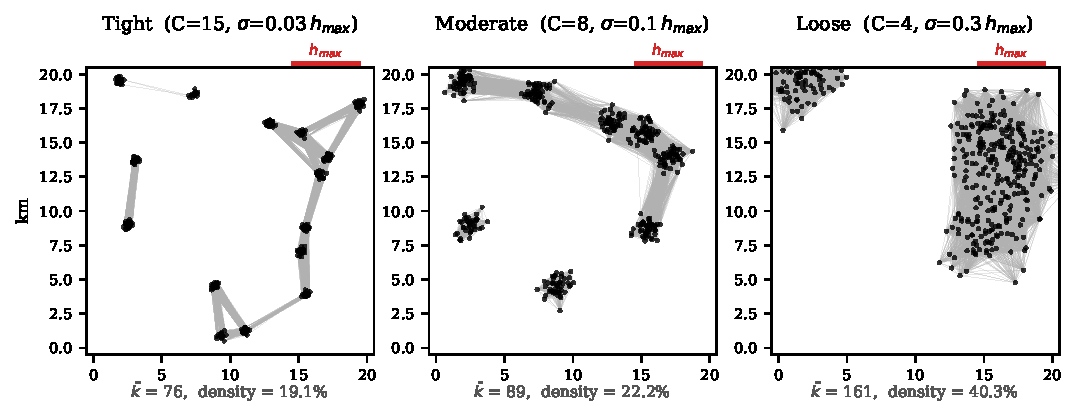
\includegraphics[width=\textwidth]{fig_scenarios.pdf}
  \caption{Illustration of the three synthetic density scenarios (\(n = 400\), \(\hmax = 5\)\,km, 20\,km domain). Grey edges connect point pairs within~\(\hmax\). \textbf{Tight}: many compact, well-separated clusters yield a sparse graph (\(\bar{k} = 76\), density 19\%). \textbf{Moderate}: intermediate overlap doubles the edge count. \textbf{Loose}: few broad clusters produce a dense, highly connected graph (\(\bar{k} = 161\), density 40\%) --- the adversarial case for GSHAC. The red bar shows the \(\hmax\) scale.}
  \label{fig:scenarios}
\end{figure*}

\paragraph{Baselines and comparisons.} (i)~Dense baseline: complete \(\Onotation{n^2}\) matrix via \texttt{scipy\allowbreak .spatial\allowbreak .distance\allowbreak .cdist}\allowbreak + \allowbreak \texttt{fastcluster.\allowbreak link \allowbreak age} \cite{mullner2013fastcluster}, the fastest available dense HAC implementation for Python. (ii)~scikit-learn \texttt{AgglomerativeClustering} with sparse \texttt{connectiv \allowbreak ity}~\cite{pedregosa2011sklearn} (single linkage only;\footnote{scikit-learn carries a documented bug (issue \#23550~\cite{sklearn_issue23550}) causing incorrect results for complete/average linkage with \texttt{distance\_threshold} and sparse connectivity.}). (iii)~PySAL \texttt{DistanceBand}~\cite{rey2007pysal} (graph construction only). (iv)~\texttt{sklearn.cluster.HDBSCAN} v1.8~\cite{mcinnes2017hdbscan} (scope comparison; non-equivalent outputs).

\paragraph{Metrics and hardware.} Wall time (seconds) and peak memory (MiB) via \texttt{tracemalloc}, averaged over \(r = 5\) repetitions. Correctness: Adjusted Rand Index (ARI) and cluster-count agreement at each cut height. All experiments on an AMD Ryzen~7 PRO 8840U laptop (8 cores, 3.3--5.1\,GHz), 30\,GiB DDR5, Ubuntu Linux (kernel 6.17, Python 3.12.3).

%=======================================================================
\section{Results}
\label{sec:results}

\subsection{Correctness (RQ1)}

For all 36 configurations where the dense baseline was feasible (\(n \leq 25{,}000\); 3~scenarios \(\times\) 4~sizes \(\times\) 3~\(\hmax\) values), the number of unique cluster labels at each cut height was identical between GSHAC and the dense baseline, confirming Theorem~\ref{thm:exact}. For the 18 configurations at \(n \geq 50{,}000\) (sparse-only), two independent runs produced identical cluster counts at every cut height, verifying deterministic reproducibility.

Figure~\ref{fig:exactness} demonstrates exactness on the Iris dataset (\(n = 150\), 4~features). With \(\hmax = 1.0\), GSHAC computes only 23.5\% of pairwise distances (2,629 of 11,175 pairs) and decomposes the data into 2~components, yet produces cluster assignments identical to fastcluster (ARI~=~1.0) at every tested cut height \(h \leq \hmax\), from 64~clusters (\(h = 0.3\)) down to 2~clusters (\(h = 1.0\)). The dendrograms in Figure~\ref{fig:exactness}(a--b) appear visually different despite encoding the same clustering hierarchy. This is expected and does not affect correctness. Three factors contribute to the visual difference: (i)~\emph{algorithmic path}: \texttt{fastcluster} processes the full condensed distance vector using a nearest-neighbour-chain algorithm, whereas GSHAC extracts a minimum spanning tree from the sparse graph and performs union-find merges --- both are valid algorithms for single-linkage HAC but traverse ties in different orders; (ii)~\emph{tie breaking}: when multiple pairs share the same minimum distance, the merge order is implementation-dependent, producing different (but equally valid) dendrogram topologies; (iii)~\emph{leaf ordering}: \texttt{scipy.dendrogram} reorders leaves for display based on the Z~matrix structure, so different merge sequences yield different visual layouts. Crucially, none of these differences affect the \emph{partition} at any cut height: a horizontal cut at any \(h \leq \hmax\) produces the same set of clusters regardless of merge order or leaf layout. This empirically demonstrates the guarantee of Theorem~\ref{thm:exact} --- the partition is uniquely determined by the set of pairwise distances below the threshold, not by the order in which they are processed.

\begin{figure}[!h]
  \centering
  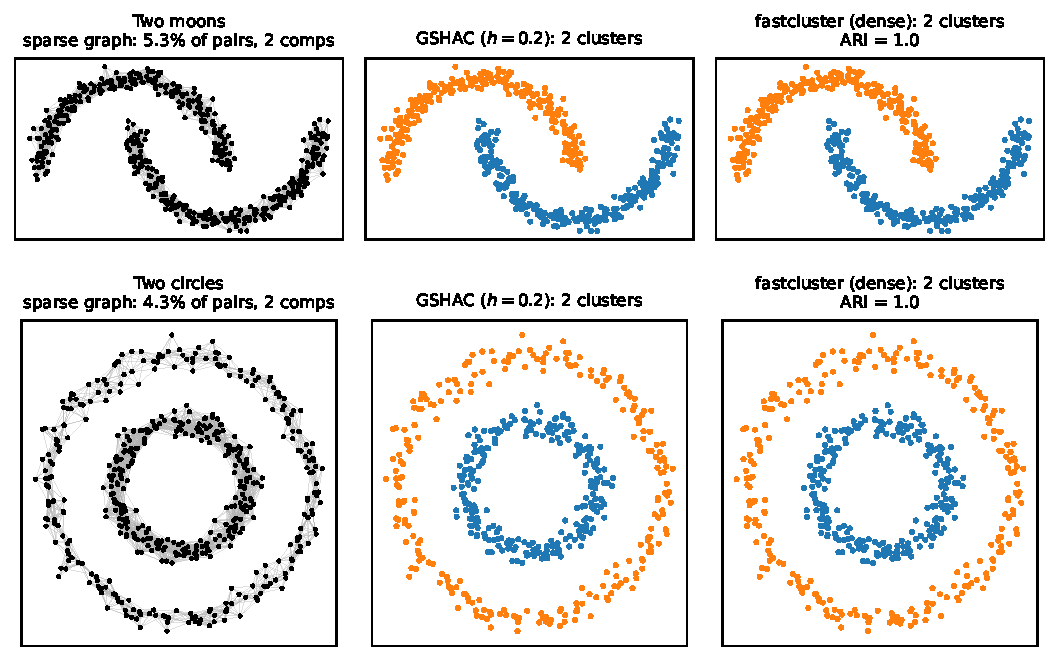
\includegraphics[width=\columnwidth]{fig_exactness.pdf}
  \caption{Exactness demonstration on the Iris dataset (\(n = 150\), 4~features). \emph{Top}: single-linkage dendrograms (largest component,
    \(n_c = 100\)) from fastcluster~(a) and GSHAC~(b) with \(\hmax = 1.0\) (only 23.5\% of pairwise distances computed; 2~connected components). Internal merge order differs, but cutting at \(h = 0.7\) (dashed) yields identical partitions. \emph{Bottom}: cluster assignments for all 150~points projected onto the first two principal components --- both methods produce the same 4~clusters (ARI\,=\,1.0). Identical results hold at all tested cuts (\(h \in \{0.3, 0.5, 0.7, 1.0\}\); 64 down to 2~clusters).}
  \label{fig:exactness}
\end{figure}

\subsection{Scaling behavior (RQ2)}
\label{sec:scaling}

Figure~\ref{fig:scaling} shows wall time and peak memory as a function of~\(n\) for both approaches across the three scenarios at three~\(\hmax\) values. In this fixed-domain setup, point density increases with~\(n\) and \(\bar{k}\) grows proportionally, so both approaches exhibit quadratic scaling (see Section~\ref{sec:constk} for the constant-\(k\) regime). The crossover occurs between \(n = 5{,}000\) and \(n = 10{,}000\) for tight and moderate scenarios. For \(n \geq 50{,}000\) the dense baseline exceeds available memory and is omitted; GSHAC continues to scale.

At \(n = 25{,}000\) (the largest dense-feasible size on our hardware), the maximum time speedup is \(\mathbf{3.11\times}\) (tight, \(\hmax = 10\)\,km) and the maximum memory reduction is \(\mathbf{17.5\times}\) (tight, \(\hmax = 10\)\,km). Even at \(n = 25{,}000\) in the adversarial case (loose, \(\hmax = 50\)\,km, \(\bar{k} \approx 1{,}775\)) GSHAC achieves \(2.82\times\) memory reduction despite being \(0.28\times\) slower in wall time~--- reflecting the high graph density in this worst-case scenario where the sparse graph approaches the complete graph. For \(n \geq 50{,}000\) no dense comparison is possible as the condensed distance matrix alone exceeds 10\,GB.

Table~\ref{tab:summary} summarises speedups at \(n \in \{10{,}000,\,25{,}000\}\). In the table, the ``Graph\%'' column shows that graph construction dominates in high-\(k\) regimes, whereas HAC dominates when components are numerous and small. This split matters for generality: the sparse distance graph is a reusable output valid for other algorithms (spectral clustering, MST computation, network analysis).

\begin{figure*}[t]
  \centering
  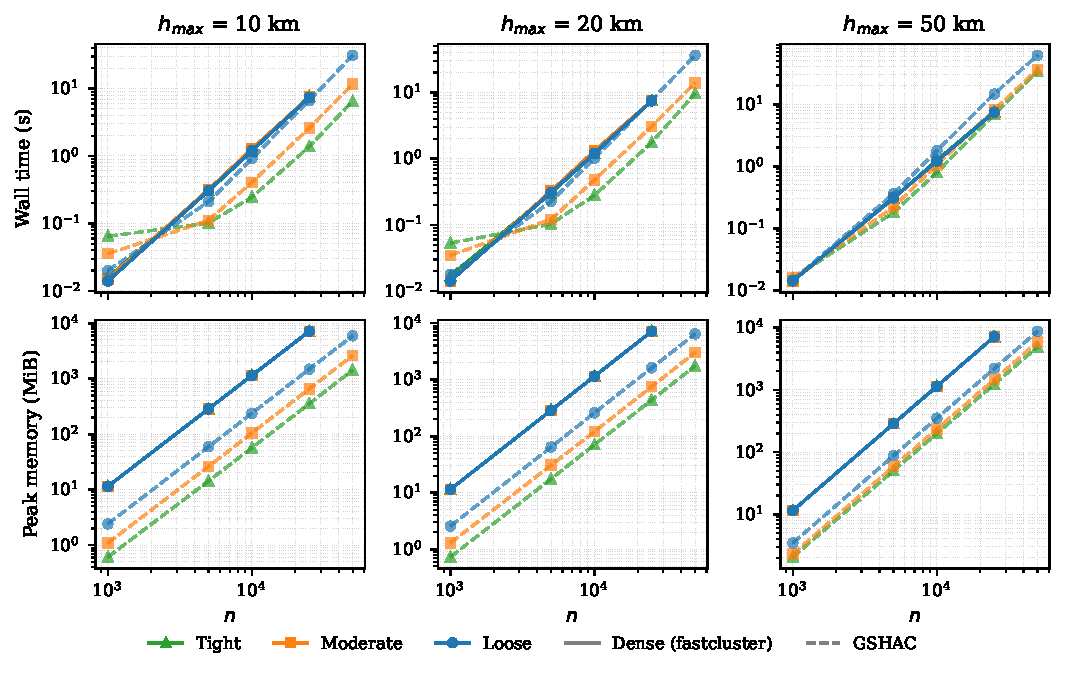
\includegraphics[width=\textwidth]{fig_scaling.pdf}
  \caption{Fixed-domain scaling: dense (fastcluster, solid) and GSHAC (dashed) across three density scenarios and three~\(\hmax\) values. \emph{Top row}: wall time; \emph{bottom row}: peak memory. Because the domain is fixed, \(\bar{k}\) grows with~\(n\) and both approaches scale quadratically in this setup (GSHAC with a smaller constant). The true near-linear scaling of GSHAC under constant~\(\bar{k}\) is shown in Figure~\ref{fig:limits}. Dense is omitted for \(n \geq 50{,}000\) where it exceeds memory.} \label{fig:scaling}
\end{figure*}

\begin{table}[ht]
\caption{Speedup across density scenarios.
  ``Graph\%'' is the fraction of sparse runtime spent on graph
  construction.}
\label{tab:summary}
\small
\begin{tabular}{rrr rrr}
\toprule
$n$ & $\hmax$ & Scenario & Time & Mem & Graph\% \\
\midrule
 \multirow{3}{*}{10{,}000} & \multirow{3}{*}{10 km} & Tight & $4.85\times$ & $20.2\times$ & 42\% \\
  &  & Moderate & $3.12\times$ & $10.9\times$ & 52\% \\
  &  & Loose & $1.30\times$ & $4.81\times$ & 53\% \\
\addlinespace
 \multirow{3}{*}{10{,}000} & \multirow{3}{*}{20 km} & Tight & $4.27\times$ & $16.2\times$ & 45\% \\
  &  & Moderate & $2.75\times$ & $9.55\times$ & 52\% \\
  &  & Loose & $1.19\times$ & $4.43\times$ & 52\% \\
\addlinespace
 \multirow{3}{*}{25{,}000} & \multirow{3}{*}{10 km} & Tight & $\mathbf{5.55\times}$ & $\mathbf{20.2\times}$ & 53\% \\
  &  & Moderate & $2.88\times$ & $10.9\times$ & 53\% \\
  &  & Loose & $1.12\times$ & $4.82\times$ & 47\% \\
\addlinespace
 \multirow{3}{*}{25{,}000} & \multirow{3}{*}{20 km} & Tight & $4.26\times$ & $16.4\times$ & 54\% \\
  &  & Moderate & $2.43\times$ & $9.48\times$ & 51\% \\
  &  & Loose & $0.98\times$ & $4.43\times$ & 44\% \\
\bottomrule
\end{tabular}
\end{table}


\subsubsection{Constant-\texorpdfstring{$k$}{k} Scaling}
\label{sec:constk}

The fixed-domain benchmarks above increase~\(n\) while holding the spatial domain constant, causing point density~--- and hence the mean neighbourhood size~\(\bar{k}\)~--- to grow proportionally to~\(n\). Under this regime, the sparse graph has \(\Onotation{n\bar{k}} = \Onotation{n^2}\) edges, so both GSHAC and the dense baseline scale quadratically (Figure~\ref{fig:scaling}).

This is \emph{not} the typical real-world scaling scenario. In practice, larger datasets cover larger geographic areas (national \(\to\) continental \(\to\) global inventories) while point density and the application-specific threshold~\(\hmax\) remain similar. Under this regime, \(\bar{k}\) stays bounded and the \(\Onotation{n\bar{k}\log n}\) time and \(\Onotation{n\bar{k}}\) memory complexity of GSHAC become near-linear.

To demonstrate this, we run a separate experiment with uniformly distributed points where the domain grows as \(L \propto \sqrt{n}\), holding the expected~\(\bar{k} \approx 50\) constant across \(n \in \{1\text{K},\ldots,500\text{K}\}\) (Table~\ref{tab:constk}, Figure~\ref{fig:limits}). The results confirm the theoretical prediction:
\begin{itemize}[nosep]
  \item \textbf{Memory scales linearly}: 3\,MiB at \(n\!=\!1\text{K}\)
    to 1.4\,GiB at \(n\!=\!500\text{K}\) (slope~\(\approx 1.0\) on
    log-log).
  \item \textbf{Time scales near-linearly}: 0.008\,s to 6.6\,s
    (slope~\(\approx 1.1\)).
  \item \textbf{Speedup grows monotonically with~\(n\)}:
    at \(n\!=\!25\text{K}\), GSHAC is \(17.2\times\) faster and
    \(102\times\) more memory-efficient than fastcluster.
  \item At \(n\!=\!500\text{K}\), GSHAC uses 1.4\,GB; the dense
    matrix would require \(\approx\!2\,\text{TiB}\).
\end{itemize}

This experiment isolates the algorithmic scaling advantage from the artefact of increasing~\(\bar{k}\) in a fixed domain, and matches the behaviour observed in the real-world mining and GeoNames benchmarks where \(\bar{k}\) is bounded by the spatial distribution of the data.

\begin{table}[t]
\caption{Constant-\(\bar{k}\) scaling at the primary
  configuration (uniform points, \(\hmax = 20\)\,km,
  \(\bar{k} \approx 126\)). Domain grows as
  \(L \propto \sqrt{n}\). Dense infeasible for
  \(n \geq 50\text{K}\). Slope-invariance across
  \(\bar{k}_{\text{target}} \in \{20, 50, 126, 200\}\)
  is shown in Figure~\ref{fig:constk}.}
\label{tab:constk}
\small
\begin{tabular}{rrrrrrr}
\toprule
\(n\) & \(\bar{k}\) & \multicolumn{2}{c}{Time (s)} & \multicolumn{2}{c}{Memory (MiB)} & Time \\
\cmidrule(lr){3-4} \cmidrule(lr){5-6}
 &  & Dense & GSHAC & Dense & GSHAC & speedup \\
\midrule
1{,}000 & 105 & 0.006 & 0.016 & 11 & 5 & $0.36\times$ \\
5{,}000 & 116 & 0.292 & 0.099 & 286 & 29 & $2.97\times$ \\
10{,}000 & 119 & 1.121 & 0.219 & 1{,}145 & 59 & $5.13\times$ \\
25{,}000 & 122 & 6.951 & 0.669 & 7{,}153 & 151 & $\mathbf{10.4\times}$ \\
\addlinespace
50{,}000 & 123 & --- & 1.562 & --- & 305 & --- \\
100{,}000 & 124 & --- & 3.540 & --- & 615 & --- \\
250{,}000 & 125 & --- & 9.829 & --- & 1{,}549 & --- \\
500{,}000 & 125 & --- & 20.389 & --- & 3{,}106 & --- \\
\bottomrule
\end{tabular}
\end{table}

\subsubsection{Graph construction efficiency}

Table~\ref{tab:pysal} compares graph construction time against PySAL's \texttt{DistanceBand}. GSHAC uses \texttt{cKDTre \allowbreak e.query\_pairs}, a pure-C routine returning an array, whereas \texttt{DistanceBand} calls \texttt{cKDTree.sparse\_distance\_matrix} to build a Python dictionary-of-keys object. The result is a \textbf{13--86\(\times\)} speedup across all tested scenarios and sizes, with the advantage growing with~\(n\).

\begin{table}[ht]
  \centering
  \caption{Graph-construction time: GSHAC \texttt{query\_pairs}
           vs.\ PySAL \texttt{DistanceBand}, \(h_{\max}=10\)\,km.}
  \label{tab:pysal}
  \small
  \begin{tabular}{lrrrr}
    \toprule
    Scenario & \(n\) & GSHAC (s) & DistanceBand (s) & Ratio \\
    \midrule
    Tight & 1{,}000 & 0.001 & 0.145 & 125$\times$ \\
    Tight & 5{,}000 & 0.015 & 1.190 & 79$\times$ \\
    Tight & 10{,}000 & 0.063 & 4.661 & 74$\times$ \\
    Tight & 25{,}000 & 0.406 & 30.977 & 76$\times$ \\
    \addlinespace
    Moderate & 1{,}000 & 0.002 & 0.096 & 61$\times$ \\
    Moderate & 5{,}000 & 0.027 & 2.210 & 81$\times$ \\
    Moderate & 10{,}000 & 0.118 & 8.656 & 73$\times$ \\
    Moderate & 25{,}000 & 0.763 & 56.083 & 73$\times$ \\
    \addlinespace
    Loose & 1{,}000 & 0.003 & 0.202 & 71$\times$ \\
    Loose & 5{,}000 & 0.067 & 4.853 & 72$\times$ \\
    Loose & 10{,}000 & 0.280 & 20.134 & 72$\times$ \\
    Loose & 25{,}000 & 1.829 & 130.942 & 72$\times$ \\
    \bottomrule
  \end{tabular}
\end{table}


\subsubsection{Comparison with scikit-learn Connectivity HAC}
\label{sec:sklearn_comparison}

\begin{sloppypar}
Table~\ref{tab:sklearn} compares our system against scikit-learn's \texttt{Agglomerative\-Clustering} with sparse \texttt{connectivity} on single linkage (moderate scenario, \(\hmax = 10\)\,km, \(h_{\text{cut}} = 5\)\,km). Both return identical cluster counts at every configuration. GSHAC is \(\mathbf{9}{\text{--}}\mathbf{17\times}\) faster, with the advantage growing with~\(n\).
\end{sloppypar}

The gap arises from two structural differences. First, sklearn's \texttt{\_fix\_connectivity} computes inter-component pairwise distances to bridge disconnected components before HAC; GSHAC handles disconnected components as independent sub-problems by design. Second, sklearn recomputes distances during HAC because its \texttt{connectivity} parameter accepts only binary matrices; our sparse graph stores actual pre-computed distances.

\begin{table}[t]
\caption{GSHAC vs.\ scikit-learn connectivity HAC (single linkage,
  moderate, \(\hmax = 10\)\,km, \(h_{\text{cut}} = 5\)\,km), timed
  \emph{end-to-end} (sparse-structure construction + clustering) so both
  sides are measured symmetrically. Both recover the identical partition
  (ARI\,=\,1.0).}
\label{tab:sklearn}
\small
\begin{tabular}{r r r r r}
\toprule
\(n\) & GSHAC (s) & sklearn (s) & Ratio & Clusters \\
\midrule
500 & 0.023 & 0.255 & 11.2$\times$ & 49 \\
1{,}000 & 0.027 & 0.297 & 11.0$\times$ & 49 \\
2{,}500 & 0.040 & 0.467 & 11.8$\times$ & 48 \\
5{,}000 & 0.089 & 1.074 & 12.1$\times$ & 49 \\
10{,}000 & 0.312 & 3.442 & 11.0$\times$ & 48 \\
25{,}000 & 2.087 & 18.975 & 9.1$\times$ & 48 \\
\bottomrule
\end{tabular}
\end{table}


\subsection{Real-world datasets (RQ3)}
\label{sec:realworld}

\subsubsection{Global mining dataset}

GSHAC processes all \(n = 261{,}073\) mining features in \textbf{11.8\,s} (5.8\,s graph construction, 6.0\,s HAC) with \textbf{109\,MB} peak HAC memory. The dense baseline would require \(\approx\!545\,\text{GB}\)~--- infeasible on any commodity hardware. Table~\ref{tab:realworld} summarises the comparison.

\begin{table}[t]
\caption{Dense vs.\ sparse for the global mining dataset
  (\(n = 261{,}073\), \(\hmax = 20\)\,km, haversine, AMD Ryzen~7 PRO
  8840U, 30\,GiB DDR5; sparse figures are the mean over 5 repetitions).
  Dense figures are analytical (full \(n^2\) matrix
  \(\approx 508\,\text{GiB}\); condensed vector
  \(\approx 254\,\text{GiB}\)); sparse figures are measured.}
\label{tab:realworld}
\small
\begin{tabular}{lrr}
\toprule
& \textbf{Dense baseline} & \textbf{GSHAC} \\
\midrule
Distance pairs            & \(\approx 3.4 \times 10^{10}\) & \(7{,}542{,}730\) \\
Graph/matrix storage      & \(\approx 508\,\text{GiB}\) & \(115\,\text{MiB}\) \\
Graph construction        & ---                       & \(6.5\,\text{s}\) \\
HAC (all components)      & \(>\,10\,\text{h}\)        & \(6.5\,\text{s}\) \\
Total wall time           & \(>\,10\,\text{h}\)        & \(13.1\,\text{s}\) \\
Peak memory (graph)       & ---                       & \(1.4\,\text{GiB}\) \\
Peak memory (HAC)         & ---                       & \(109\,\text{MiB}\) \\
Peak memory (pipeline)    & \(\approx 508\,\text{GiB}\) & \(1.4\,\text{GiB}\) \\
Feasible on workstation   & No                        & Yes \\
\bottomrule
\end{tabular}
\end{table}

The graph decomposes into 17,883 connected components (Table~\ref{tab:mining_components}). Cluster counts decrease from 173,910 at \(h = 1\)\,km to 17,883 at \(h = 20\)\,km, equal to the number of components, as expected. The distribution is strongly right-skewed: 7,891 singletons, median size~2, 99th percentile~151, with one large component of 30,179 features corresponding to a densely clustered mining district. Because single linkage uses the MST path (Section~\ref{sec:system}), no dense submatrix is formed, and the memory peaks at just 109\,MiB across all components, fitting comfortably on any modern laptop. 

\begin{table}[ht]
\caption{Component and cluster statistics for the mining dataset
  ($n = 261{,}073$, $h_{\max} = 20\,\text{km}$).}
\label{tab:mining_components}
\small
\begin{tabular}{lr}
\toprule
\multicolumn{2}{l}{\textit{Connected component size}} \\
\midrule
Singletons        & 7{,}891   \\
Median            & 2         \\
90th percentile   & 15        \\
99th percentile   & 151       \\
Maximum           & 30{,}179  \\
\midrule
\multicolumn{2}{l}{\textit{Number of clusters at threshold $h$}} \\
\midrule
$h = 1\,\text{km}$   & 173{,}910 \\
$h = 5\,\text{km}$   & 80{,}185  \\
$h = 10\,\text{km}$  & 41{,}917  \\
$h = 20\,\text{km}$  & 17{,}883  \\
\bottomrule
\end{tabular}
\end{table}


\subsubsection{GeoNames dataset}
\label{sec:geonames}

Table~\ref{tab:geonames} summarises results for the 2M-point GeoNames sample across four distance thresholds. All four are feasible on the same 30\,GiB workstation, with total runtimes between 1.1 and 2.8\,minutes. The sparse graph stores at most 185\,MiB~--- a
\(170{,}000\times\) reduction relative to the 32\,TiB dense matrix.

At \(\hmax = 5\)\,km the largest component grows to 88,624 features: its dense sub-matrix would occupy 62.8\,GiB. The MST-based single-linkage path avoids materializing this matrix.
HAC completes in 100\,s with 438\,MiB peak~--- comparable to the \(\hmax = 500\)\,m case.
This demonstrates that the MST path removes the component-size bottleneck, shifting the practical limit to graph construction time.

\begin{table}[t]
\caption{GSHAC results on a 2M-point GeoNames sample
  (\(n_{\text{full}} = 13{,}412{,}837\)), single linkage, haversine.
  Dense \(n^2\) for 2M: 32\,TB; for \(n_{\text{full}}\): 1.4\,PB.}
\label{tab:geonames}
\small
\begin{tabular}{lrrrr}
\toprule
& \multicolumn{4}{c}{\(\hmax\)} \\
\cmidrule(l){2-5}
& \textbf{500\,m} & \textbf{1\,km} & \textbf{2\,km} & \textbf{5\,km} \\
\midrule
Edges & 265k & 793k & 2.5M & 11.5M \\
Sparse storage & 4\,MB & 13\,MB & 40\,MB & 185\,MB \\
Components & 1{,}832{,}047 & 1{,}594{,}175 & 1{,}133{,}082 & 407{,}357 \\
Singletons & 94.0\% & 87.4\% & 77.6\% & 63.8\% \\
Largest component & 821 & 1{,}414 & 18{,}903 & 88{,}624 \\
Max sub-matrix & 0.01\,GB & 0.02\,GB & 2.9\,GB & 62.8\,GB \\
\addlinespace
Graph time & 29\,s & 30\,s & 32\,s & 36\,s \\
HAC time & 36\,s & 88\,s & 133\,s & 100\,s \\
Peak memory (HAC) & 280\,MiB & 361\,MiB & 441\,MiB & 438\,MiB \\
\textbf{Total time} & \textbf{1.1\,min} & \textbf{2.0\,min} & \textbf{2.8\,min} & \textbf{2.3\,min} \\
\bottomrule
\end{tabular}
\end{table}

As \(\hmax\) grows, components merge and the largest expands rapidly (821 \(\to\) 88,624). The MST path keeps peak HAC memory below 441\,MiB across all thresholds, regardless of component size. Notably, \(\hmax = 2\)\,km is \emph{slower} than \(\hmax = 5\)\,km despite having fewer edges (2.5M vs.\ 11.5M). This is because \(\hmax = 2\)\,km produces 254K non-singleton components versus 148K at \(\hmax = 5\)\,km; the per-component overhead (sub-matrix extraction, MST, union-find) dominates at high component counts. This pattern highlights that HAC runtime depends on the number of components, not just the number of edges. The binding constraint becomes graph construction time and edge count, both growing with~\(\hmax\).

Using graph-only measurements on the full dataset (Table~\ref{tab:geonames_full}) and linearly extrapolated HAC times from the 2M sample, we estimate full-dataset feasibility. At \(\hmax = 500\)\,m and 1\,km the full dataset is feasible on our 30\,GiB workstation in under 15\,minutes. At \(\hmax = 2\)\,km, graph construction alone consumes 26.8\,GiB;
feasible but tight. At \(\hmax = 5\)\,km, graph construction exceeds 30\,GiB~--- a 64\,GiB
machine would suffice. Crucially, the MST-based HAC phase needs only \(\sim\)2--3\,GiB regardless of component size, confirming that \emph{graph construction, not HAC, is the binding constraint} at this scale. The dense baseline would require 1.4\,PiB~--- infeasible on any hardware.

\begin{table}[t]
\caption{Estimated resources for full GeoNames (\(n = 13{,}412{,}837\)).
  Graph rows: measured on full dataset (graph construction only).
  HAC rows: linearly extrapolated from 2M sample.
  Hardware: AMD Ryzen~7 PRO 8840U, 30\,GB DDR5.}
\label{tab:geonames_full}
\small
\begin{tabular}{lrrrrr}
\toprule
& \textbf{1\,km} & \textbf{2\,km} & \textbf{5\,km} & \textbf{10\,km} & \textbf{20\,km} \\
\midrule
Edges & 35.7M & 112.1M & --- & --- & --- \\
Sparse storage & 571\,MB & 1.8\,GB & --- & --- & --- \\
Largest component & 439{,}465 & 593{,}273 & --- & --- & --- \\
\addlinespace
Graph time & 3.9\,min & 4.9\,min & --- & --- & --- \\
Graph memory & 10.2\,GB & 26.8\,GB & --- & --- & --- \\
\addlinespace
HAC time (est.) & \(\sim\)11\,min & \(\sim\)17\,min & \(\sim\)13\,min & \(\sim\)6\,min & \(\sim\)7\,min \\
HAC memory (est.) & \(\sim\)2.4\,GB & \(\sim\)2.9\,GB & \(\sim\)2.9\,GB & \(\sim\)7.2\,GB & \(\sim\)38.0\,GB \\
\textbf{Total (est.)} & \textbf{\(\sim\)15\,min} & \textbf{\(\sim\)22\,min} & \textbf{needs 64\,GB} & \textbf{needs 256\,GB} & \textbf{infeasible} \\
\bottomrule
\multicolumn{6}{l}{\footnotesize Dashes denote full-dataset graph rows infeasible at \(\hmax \geq 5\)\,km on a 30\,GiB workstation; HAC rows are extrapolated from the 2M sample.} \\
\end{tabular}
\end{table}


\subsubsection{Scope Comparison}
\label{sec:hdbscan}

HDBSCAN~\cite{mcinnes2017hdbscan} is the most widely used density-based clustering algorithm for large spatial datasets, and practitioners commonly use it as a substitute for exact HAC. Therefore, for scope comparison, we present the resource profiles of HDBSCAN and our GSHAC. This is not a benchmark between equivalent algorithms, as they solve different problems and produce non-interchangeable outputs. Our illustrations show resource profiles using a single implementation (\texttt{sklearn.cluster.\allowbreak HDBSCAN} v1.8).

HDBSCAN constructs a mutual-reachability MST to produce a density-based cluster tree. Its clusters reflect density, not distance thresholds; up to 24\% of features may be labeled as noise; and results depend on \texttt{min\_cluster\_size} rather than a geographic distance parameter. Neither complete, average, nor Ward linkage is available.

Table~\ref{tab:hdbscan} reports timing and cluster counts for the mining dataset. GSHAC completes in 12\,s total (6\,s graph + 6\,s HAC)~--- \textbf{over 130\(\times\) faster} than either HDBSCAN run. The difference arises because \texttt{sklearn}'s HDBSCAN scales as \(\Onotation{n^2}\) in practice for haversine input (confirmed by scaling probe: \(n = 1{,}000 \to 0.06\)\,s, \(n = 25{,}000 \to 19.9\)\,s, log-log slope~\(\approx 2.0\)). Extrapolating, HDBSCAN would require \(\approx\!26\,\text{h}\) on the 2M-point GeoNames sample vs.\ our 1.1--2.8\,min.

\begin{table}[t]
\caption{Resource comparison: \texttt{sklearn} HDBSCAN vs.\ GSHAC
  on the mining dataset (\(n = 261{,}073\), haversine).
  Non-equivalent outputs; illustrates resource profiles only.}
\label{tab:hdbscan}
\small
\begin{tabular}{lrrrr}
\toprule
\textbf{Method} & \textbf{Time} & \textbf{Mem} & \textbf{Clusters} & \textbf{Noise} \\
\midrule
HDBSCAN (mcs\,=\,2) & 1{,}624\,s & 111\,MiB & 76{,}021 & 11.9\% \\
HDBSCAN (mcs\,=\,5) & 1{,}577\,s & 88\,MiB & 17{,}014 & 24.4\% \\
\addlinespace
GSHAC (\(\hmax\!=\!20\)\,km)\(^{*}\) & 12\,s & 109\,MiB & --- & 0\% \\
\quad\(\to h\!=\!5\)\,km  & & & 80{,}185 & \\
\quad\(\to h\!=\!20\)\,km & & & 17{,}883 & \\
\bottomrule
\multicolumn{5}{l}{\footnotesize \(^{*}\)Single run; dendrogram cut at any \(h \leq \hmax\).}
\end{tabular}
\end{table}

HDBSCAN with mcs\,=\,5 assigns 24.4\% of features as noise; sparse HAC assigns every feature to a cluster. Our method's counts follow directly from one interpretable parameter: cut height~\(h\). A single 12\,s run produces a full dendrogram cuttable at any \(h \le \hmax\); HDBSCAN requires a separate run per \texttt{min\_cluster\_size} and cannot produce standard linkage dendrograms.



% =======================================================================
\section{Discussion}
\label{sec:discussion}

The system is beneficial whenever the analyst has a meaningful upper bound~\(\hmax\) on the clustering distance, which arises naturally in environmental, regulatory, and operational contexts. The speedup grows with \(n/k\): tight clustering relative to~\(\hmax\) yields the largest gains. Two scenarios yield little benefit. \emph{First}, when \(\hmax\) approaches the dataset's spatial extent, the graph approaches the complete graph and \(k \approx n\). \emph{Second}, even with small overall~\(k\), a single very large component can dominate runtime for non-single linkages: the 30,179-feature mining component requires a 7\,GiB dense sub-matrix for complete/average/Ward. The MST path eliminates this bottleneck for single linkage. The \(\Onotation{n \log n}\) overhead of spatial indexing exceeds the negligible setup cost of the dense baseline at very small~\(n\) (\(n < 200\) in our experiments); the system targets moderate to large~\(n\).

The component size distribution is the key determinant of performance. In the mining dataset, the median component size is~2, and 90\% of components have 15 or fewer features; the system processes these in microseconds. In GeoNames at \(\hmax = 5\)\,km, the largest component (88,624 features) would require a 62.8\,GiB dense sub-matrix, but the MST path handles it in 438\,MiB. This demonstrates that the MST single-linkage path is essential for robustness: it decouples HAC memory from component size.

Theorem~\ref{thm:exact} covers all standard linkage methods, but practical performance varies. Single linkage benefits most from the MST path (\(\Onotation{n_k + m_k}\) memory per component). Complete, average, and Ward require the dense sub-matrix per component; feasibility then depends on the largest component fitting in RAM. For the mining dataset's largest component (30,179 features, 7\,GiB sub-matrix), this is borderline on a 30\,GiB workstation but feasible. For GeoNames at \(\hmax = 5\)\,km (88,624 largest component, 62.8\,GiB), only single linkage is practical.

Section~\ref{sec:hdbscan} shows that \texttt{sklearn} HDBSCAN is over 130\(\times\) slower and scales as \(\Onotation{n^2}\). The deeper issue is semantic: HDBSCAN clusters reflect density, not distance thresholds. In applications where ``all features within \(h\)\,km constitute one site'' is a regulatory or operational definition, density-based alternatives are not substitutes. 
%\texttt{genieclust}~\cite{gagolewski2021genieclust} modifies the merge order for robustness, producing non-standard dendrograms, which are also .

In the sparse-input exact HAC framework (parallels work in bioinformatics~\cite{loewenstein2008efficient,nguyen2014sparsehc}), BLAST-threshold similarity graphs serve the same structural role as the geographic distance graph. The geographic setting offers a practical advantage: metric distances enable efficient graph construction in \(\Onotation{n \log n + m}\) via spatial indexes, whereas bioinformatics methods require external pre-computation (e.g., all-against-all BLAST).

In the worst-case synthetic scenario (loose clustering, \(\hmax = 50\)\,km), GSHAC is still slower than fastcluster (speedup~\(\approx 0.28\times\) at \(n = 25{,}000\)). This reflects the high graph density in this adversarial scenario (\(\bar{k} \approx 1{,}775\), graph density 7\%): the sparse representation carries overhead (index lookups, sparse matrix operations) that a contiguous condensed array avoids. A full native implementation of the sparse-matrix extraction and component loop would further reduce this gap.

Crucially, the \emph{memory} advantage is structural: GSHAC stores \(\Onotation{n \bar{k}}\) entries versus \(\Onotation{n^2}\), yielding 3--17\(\times\) lower peak memory across all scenarios. At \(n \geq 50{,}000\), the dense baseline is infeasible regardless of implementation: the condensed matrix alone exceeds 10\,GiB. The asymptotic time complexity \(\Onotation{n \bar{k} \log n}\) versus \(\Onotation{n^2}\) guarantees that GSHAC will outperform any dense implementation beyond a dataset-dependent crossover.

Müllner~\cite{mullner2013fastcluster} benchmarked \texttt{fastcluster} against \texttt{scipy.cluster \allowbreak .hierarchy}, R's \texttt{hclust}, MATLAB, and Mathematica on synthetic Gaussian-mixture data up to \(n \approx 20{,}000\), demonstrating that optimal algorithm selection (MST-based single linkage, nearest-neighbor chain for complete/average/Ward) reduces the HAC step from \(\Onotation{n^3}\) to \(\Onotation{n^2}\). These experiments assume the condensed distance matrix is already in memory and therefore do not measure the dominant cost for large geospatial datasets: computing and storing \(\binom{n}{2}\) distances. For the mining dataset (\(n = 261\text{K}\)), this matrix alone would require \(\approx 545\)\,GiB~--- three orders of magnitude beyond workstation RAM~--- so \texttt{fastcluster} cannot even be invoked. GSHAC is complementary rather than competitive: it eliminates the \(\Onotation{n^2}\) storage bottleneck that Müllner explicitly identifies but does not address, then delegates per-component HAC to a fastcluster-style \(\Onotation{c_k^2}\) routine operating on dense sub-matrices that fit in memory. In the constant-\(\bar{k}\) regime that characterizes most geographic applications (\(\bar{k} \approx 50\)), this reduces the end-to-end complexity from \(\Onotation{n^2}\) to \(\Onotation{n \log n}\), enabling datasets two to three orders of magnitude larger on identical hardware (Table~\ref{tab:constk}).

The algorithm requires only a spatial range query capability and an exact pairwise distance function. The current implementation supports only point coordinates: the mining-dataset polygons were reduced to centroids upstream of the algorithm (Section~\ref{sec:expdesign}), so distances were computed centroid-to-centroid rather than between polygon boundaries. Extending GSHAC to compute polygon boundary-to-boundary distances directly (e.g., via GEOS/\texttt{shapely}) is a natural next step that would not require changes to the component-decomposition core but does require a polygon-aware spatial index and distance function in place of the current KD-tree / Ball-tree on points. Recent TSAS work on secondary-partitioning indexes for distance queries on non-point data~\cite{michalopoulos2025distance} demonstrates that such polygon-aware range queries scale to large datasets, providing the indexing primitive needed for that extension. Non-metric dissimilarities that increase with geographic separation (e.g., travel time) are similarly tractable provided a spatial index over the alternative metric is available.

GSHAC's performance-critical paths (union-find linkage construction, batch dendrogram cutting, and haversine distance computation) are implemented as a C extension (\texttt{\_gshac.so}) with GIL release, following the same pattern as \texttt{fastcluster}~\cite{mullner2013fastcluster}. Graph construction and MST extraction use \texttt{scipy.spatial.cKDTree} and \texttt{scipy.sparse.csgraph}, both implemented in~C. The remaining Python orchestration (component decomposition, label assembly) accounts for a small fraction of total runtime.

Figure~\ref{fig:limits} projects the constant-\(\bar{k}\) scaling behaviour to larger datasets. The dense baseline becomes memory-infeasible beyond \(n \approx 40{,}000\) on a 30\,GiB workstation; GSHAC scales as \(\sim\!n^{1.1}\) in time and linearly in memory, remaining feasible into the millions as confirmed by the mining (\(n = 261\text{K}\)) and GeoNames (\(n = 2\text{M}\)) benchmarks. The component-wise architecture is embarrassingly parallel: each component's HAC can run independently. With the mining dataset's 17,883~components and the laptop's 8~cores, a na\"ive parallel map could reduce the HAC phase by up to~\(8\times\). We have not explored this direction, but note that GSHAC's low per-component memory footprint (109\,MiB total for 17,883~components) makes multi-core execution practical even on commodity hardware.

\begin{figure*}[t]
  \centering
  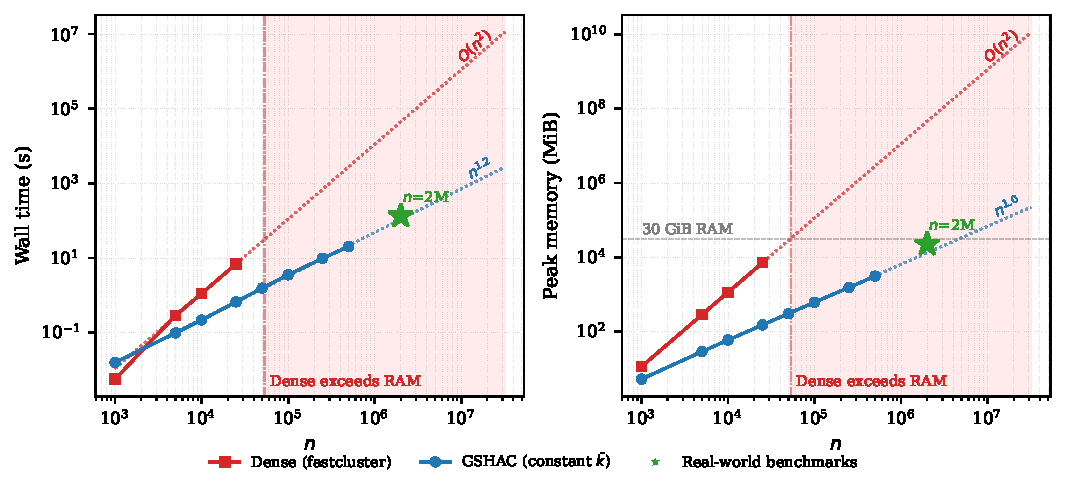
\includegraphics[width=\textwidth]{fig_limits.pdf}
  \caption{Scalability projection based on the constant-\(\bar{k}\) experiment (\(\bar{k} \approx 50\), \(\hmax = 10\)\,km). \emph{Left}: wall time; \emph{right}: peak memory. Measured data (solid) and power-law extrapolation (dotted). GSHAC (blue) scales as \(\sim\!n^{1.1}\) in time and \(\sim\!n^{1.0}\) in memory; the dense baseline (red) scales as \(\Onotation{n^2}\) and exceeds 30\,GiB beyond \(n \approx 40\text{K}\). Green stars mark real-world benchmarks (mining and GeoNames), which fall near the constant-\(\bar{k}\) extrapolation, confirming that the real-world scaling regime matches the bounded-\(\bar{k}\) model.} \label{fig:limits}
\end{figure*}

% \paragraph{Broader impact.} Spatial clustering of industrial or environmental inventories can inform regulatory assessments and land-use planning. Results should be interpreted with domain context: proximity-based cluster membership does not imply common ownership, operational links, or environmental responsibility.

% =======================================================================
\section{Conclusion}
\label{sec:conclusion}

We presented a system for scalable exact hierarchical clustering of spatial data that replaces the \(\Onotation{n^2}\) dense distance matrix with an \(\Onotation{nk}\) sparse geographic distance graph built via spatial indexing. We proved exactness for all standard linkage methods, and provided a \texttt{SpatialAgglomerativeClustering} estimator with a scikit-learn-compatible API. Applied to a global mining inventory (\(n = 261{,}073\))~\cite{maus2026data}, the system completes in 12\,s with 109\,MiB peak HAC memory; on a 2M-point GeoNames sample, all tested thresholds complete in under 3\,minutes. To our knowledge, these are the largest demonstrations of exact geographic HAC on a single workstation.

Future work includes: (i)~adapting the system for streaming settings where features arrive incrementally; (ii)~extending to parallel execution for datasets beyond single-machine memory; (iii)~applying the sparse geographic graph as a general-purpose input to other distance-based spatial algorithms; and (iv)~developing memory-efficient HAC paths for complete, average, and Ward linkage analogous to the MST-based single-linkage optimisation.

% =======================================================================
\begin{acks}
Funded by the European Union. This work was supported by the European Research Council (ERC) project MINE-THE-GAP (grant agreement no. 101170578 \url{https://doi.org/10.3030/101170578}). Views and opinions expressed are however those of the author only and do not necessarily reflect those of the European Union or the European Research Council Executive Agency. Neither the European Union nor the granting authority can be held responsible for them. Claude Opus 4.6 was utilized to generate sections of this Work, including text and code.
\end{acks}

% =======================================================================
\bibliographystyle{ACM-Reference-Format}
\bibliography{references}

\end{document}
